\chapter{数理统计的基础知识}
在前六章,我们讨论了概率论的基础知识,
即对随机变量所代表的客观随机现象的统计规律性的讨论.
在概率论中,随机变量\(X\)的分布都是已知的,或假定是已知的,
从而可以求出其数字特征以及讨论有关的问题.
但在实际生活中却并非如此.

在本章,我们介绍数理统计方法(mathematical methods of statistics)的基本概念,
即通过采集样本、进行试验,初步地研究服从未知分布的随机变量的相关问题.

\section{总体与样本}
\begin{definition}
在数理统计中,我们把研究对象的全体称为\DefineConcept{总体}(population),
把总体中的每个成员称为\DefineConcept{个体}(individual).
\end{definition}

如果总体中个体数是有限的,那么称这个总体为\DefineConcept{有限总体};
反之,称这个总体为\DefineConcept{无限总体}.

在数理统计中,我们研究的不是总体的全部属性,而是总体的某项数量指标.
这项数量指标可以用一个随机变量或其对应的一个分布来刻画.
因此约定以后提到总体时,将其表记为“总体\(X\)”或“总体\(F(x)\)”.

在抽样试验前,\(n\)个个体的特征\(\{X_n\}\)是与总体同分布的随机变量;
而在抽样试验后,是\(n\)个数据\(\AutoTuple{x}{n}\).
而一般在总体中抽取的这一小部分个体要对总体有充分的代表性,需要满足以下两个条件:
\begin{enumerate}
	\item {\bf 随机性},
	即总体中每个个体都有同等机会被抽取到,
	通常可用编号抽签的方法或用随机数表来实现;
	\item {\bf 独立性},
	各次抽取必须是相互独立的,即各个个体是否被抽取到彼此独立的.
\end{enumerate}

\begin{definition}
设随机变量\(\AutoTuple{X}{n}\)与总体\(X\)独立同分布,
那么我们把\(\AutoTuple{X}{n}\)称为%
“一个来自总体\(X\)的\DefineConcept{简单随机样本}(simple random sample)”,
简称\DefineConcept{样本}(sample);
还称“这个样本的\DefineConcept{样本容量}(sample size)是\(n\)”.
而\(\AutoTuple{X}{n}\)的取值\(\AutoTuple{x}{n}\)叫做\DefineConcept{样本观测值}.
\end{definition}

从总体中进行有放回地抽样,得到的显然是简单随机样本.
从有限总体中进行不放回地抽样,虽然不是简单随机样本,但当总体个体数\(N\)很大而样本容量\(n\)较小(通常要求\(n/N \leq 0.1\)),则可以近似地看作是有放回抽样,因而近似看作是简单随机抽样,即近似地得到简单随机样本.

若将样本看作一个\(n\)维随机变量\((\AutoTuple{X}{n})\),则可求出其概率分布或密度.

当总体\(X\)是离散型随机变量,
且有分布律\(P(X = x) = p(x)\),
则样本\((\AutoTuple{X}{n})\)的分布律为\[
	P(X_1=x_1,X_2=x_2,\dotsc,X_n=x_n)
	= \prod_{i=1}^n P(X_i=x_i).
\]

当总体\(X\)是连续型随机变量,
且有密度函数\(f(x)\),
则样本\((\AutoTuple{X}{n})\)的密度函数为\[
	f(\AutoTuple{x}{n}) = \prod_{i=1}^n f(x_i).
\]

\begin{example}
总体\(X \sim e(\lambda)\),
\(\AutoTuple{X}{n}\)为来自总体\(X\)的样本.
\def\P{P(\min\{\AutoTuple{X}{n}\}>3)}
求\(\P\).
\begin{solution}
\def\intx{\int_3^{+\infty}}
\def\into{\intx \intx \dotso \intx}
\def\ddx{\dd{x_1} \dd{x_2} \dotsm \dd{x_n}}
\begin{align*}
	&\hspace{-20pt}\P \\
	&= P(X_1>3,X_2>3,\dotsc,X_n>3) \\
	&= \into f(\AutoTuple{x}{n}) \ddx \\
	&= \into f(x_1) f(x_2) \dotsm f(x_n) \ddx \\
	&= \left( \intx \lambda e^{-\lambda x_1} \dd{x_1} \right)^n
	= e^{-3n\lambda}.
\end{align*}
\end{solution}
\end{example}

\section{常见统计分布}
\(\x\)分布、\(t\)分布和\(F\)分布在数理统计中与正态分布一起构成四个最基本、最重要的分布.
下面逐一介绍前三个分布.

\subsection{\texorpdfstring{\(\x\)}{卡方}分布}
\begin{definition}\label{definition:数理统计的基础知识.卡方分布的定义}
\(\AutoTuple{X}{n}\)独立同服从标准正态分布\(N(0,1)\),
称随机变量\begin{equation}
	\x = \sum_{i=1}^n{X_i^2}
\end{equation}
所服从的分布为
“自由度为\(n\)的 \DefineConcept{\(\x\)分布}”
\footnote{念作“卡方分布”.},
记为\(\x \sim \x(n)\).
\end{definition}

\begin{figure}[ht]
	\centering
	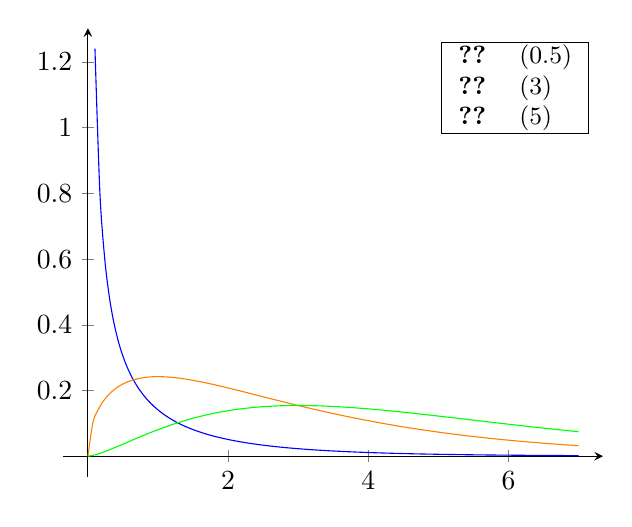
\begin{tikzpicture}
		\begin{axis}[
			name=ChiSquareDistribution,
			axis y line=middle,
			axis x line=middle,
			enlarge x limits=0.05,
			enlarge y limits=0.05,
			xscale=1,
		]
			\def\plotCSDPDF#1#2#3{\addplot[color=#3,samples=100,smooth,domain=.1:7]{%首次定义
				x^(#1-1)*exp(-x/2)/(2^(#1)*#2)
			}}%
			\plotCSDPDF{.25}{3.62561}{blue};\label{pgfplots:卡方分布.Chi^2(.5)}
			\def\plotCSDPDF#1#2#3{\addplot[color=#3,samples=100,smooth,domain=0:7]{%重新定义
				x^(#1-1)*exp(-x/2)/(2^(#1)*#2)
			}}%
			\plotCSDPDF{1.5}{0.886227}{orange};\label{pgfplots:卡方分布.Chi^2(3)}
			\plotCSDPDF{2.5}{1.32934}{green};\label{pgfplots:卡方分布.Chi^2(5)}
		\end{axis}
		\node[draw,fill=white,inner sep=0pt,below left=0.5em]
		at(ChiSquareDistribution.north east){\small\begin{tabular}{cl}
			\ref{pgfplots:卡方分布.Chi^2(.5)} & \(\x(0.5)\) \\
			\ref{pgfplots:卡方分布.Chi^2(3)} & \(\x(3)\) \\
			\ref{pgfplots:卡方分布.Chi^2(5)} & \(\x(5)\) \\
		\end{tabular}};
	\end{tikzpicture}
	\caption{\(\x\)分布的密度函数}
\end{figure}

\begin{theorem}\label{theorem:数理统计的基础知识.卡方分布的密度函数}
\(\x(n)\)分布等价于\(\Gamma\left(\frac{n}{2},\frac{1}{2}\right)\)分布,
其密度函数为\begin{equation}
	f(x,n) = \left\{ \begin{array}{cl}
		\frac{1}{2^{n/2} \Gamma(n/2)} x^{\frac{n}{2}-1} e^{-\frac{x}{2}}, & x > 0, \\
		0, & x \leq 0.
	\end{array} \right.
\end{equation}
\begin{proof}
首先求\(Z=X_1^2\)的分布.
由于\(Z\)非负,故当\(z \leq 0\)时,
\(P(Z \leq z) = 0\);
当\(z > 0\)时,\(Z\)的分布函数为\[
	F_Z(z) = P(Z \leq z)
	= P(X_1^2 \leq z)
	= P(-\sqrt{z} \leq X_1 \leq \sqrt{z})
	= F_{X_1}(\sqrt{z}) - F_{X_1}(-\sqrt{z}),
\]
相应的密度函数为\[
	f_Z(z) = \frac{1}{2} z^{-\frac{1}{2}} \left[
		f_{X_1}(\sqrt{z}) + f_{X_2}(-\sqrt{z})
	\right],
\]
其中\(f_{X_1}(x) = (2\pi)^{-\frac{1}{2}} \exp(\frac{-x^2}{2})\)为标准正态分布的密度函数,
代入即得\[
	f_Z(z) = \left\{ \begin{array}{cl}
		\frac{1}{\sqrt{2\pi}} z^{-\frac{1}{2}} e^{-\frac{z}{2}}, & z>0, \\
		0, & z \leq 0.
	\end{array} \right.
\]
这正是\(\Gamma\left(\frac{1}{2},\frac{1}{2}\right)\)的密度函数.

又因为\(\AutoTuple{X}{n}\)独立同分布,
所以\(\AutoTuple{X^2}{n}\)也独立同分布于\(\Gamma\left(\frac{1}{2},\frac{1}{2}\right)\).

再由~\hyperref[theorem:多维随机变量及其分布.伽马分布的可加性1]{\(\Gamma\)分布的可加性}可知
\(\x = X_1^2+X_2^2+\dotsb+X_n^2\)服从\(\Gamma\left(\frac{n}{2},\frac{1}{2}\right)\).
\end{proof}
\end{theorem}

\begin{corollary}\label{theorem:数理统计的基础知识.卡方分布的数字特征}
设\(\x \sim \x(n)\),则
\begin{gather}
	E(\x) = n, \\
	D(\x) = 2n.
\end{gather}
\end{corollary}

\begin{theorem}[可加性]\label{theorem:数理统计的基础知识.卡方分布的可加性1}
设\(\x_1 \sim \x(n_1)\),\(\x_2 \sim \x(n_2)\),
且\(\x_1\)与\(\x_2\)相互独立,则\begin{equation}
	\x_1 + \x_2 \sim \x(n_1+n_2).
\end{equation}
\begin{proof}
因为\[
	\x(n_1) = \Gamma\left(\frac{n_1}{2},\frac12\right), \qquad
	\x(n_2) = \Gamma\left(\frac{n_2}{2},\frac12\right),
\]
所以,根据\hyperref[theorem:多维随机变量及其分布.伽马分布的可加性1]{伽马分布的可加性}可知\[
	\x_1 + \x_2 \sim \Gamma\left(\frac{n_1+n_2}{2},\frac12\right)
	= \x(n_1+n_2).
	\qedhere
\]
\end{proof}
\end{theorem}

\begin{corollary}\label{theorem:数理统计的基础知识.卡方分布的可加性2}
设随机变量序列\(\x_k \sim \x(n_k)\ (k=1,2,\dotsc,n)\),
且\(\x_1,\x_2,\dotsc,\x_n\)相互独立,则\begin{equation}
	\sum_{k=1}^n \x_k \sim \x\left(\sum_{k=1}^n{n_k}\right).
\end{equation}
\end{corollary}

\subsection{\texorpdfstring{\(t\)}{t}分布}
\begin{definition}
设随机变量\(X \sim N(0,1)\),\(Y \sim \x(n)\),
且\(X\)与\(Y\)相互独立,称随机变量\begin{equation}
	t = \frac{X}{\sqrt{Y/n}}
\end{equation}
所服从的分布为
“自由度为\(n\)的~\DefineConcept{\(t\)分布}”
\footnote{又作“学生氏分布”.},
记为\(t \sim t(n)\).
\end{definition}

\begin{theorem}\label{theorem:数理统计的基础知识.学生氏分布的密度函数}
\(t\)分布的密度函数为\begin{equation}
	t(x,n) = \frac{
		\Gamma\left(\frac{n+1}{2}\right)
	}{
		\sqrt{n\pi} \cdot \Gamma\left(\frac{n}{2}\right)
	}
	\left(1+\frac{x^2}{n}\right)^{-\frac{n+1}{2}},
	\quad x \in \mathbb{R}.
\end{equation}
\end{theorem}

由于\(t\)分布的密度函数\(t(x,n)\)是偶函数,容易验证:
当\(n=1\)时\(t\)分布的数学期望\(E(t)\)不存在,
而当\(n \geq 2\)时数学期望\(E(t)=0\).

当自由度\(n\to\infty\)时,有\[
	\lim_{n\to\infty} t(x,n) = \frac{1}{\sqrt{2\pi}} e^{-\frac{x^2}{2}},
	\quad x \in \mathbb{R}.
\]
当\(n\)充分大时(通常需要\(n \geq 45\)),
\(t\)分布就近似于标准正态分布\(N(0,1)\).

\subsection{\texorpdfstring{\(F\)}{F}分布}
\begin{definition}
设随机变量\(X \sim \x(n)\),\(Y \sim \x(m)\),且\(X\)与\(Y\)独立,
称随机变量\begin{equation}
	F=\frac{X/n}{Y/m}
\end{equation}
所服从的分布为
“自由度为\((n,m)\)的 \DefineConcept{\(F\)分布}”,
记为\(F \sim F(n,m)\),
其中\(n\)称为\DefineConcept{第一自由度}(或\DefineConcept{分子自由度}),
\(m\)称为\DefineConcept{第二自由度}(或\DefineConcept{分母自由度}).
\end{definition}

\begin{proposition}
\(F \sim F(n,m) \implies \frac{1}{F} \sim F(m,n)\).
\end{proposition}

\begin{theorem}
\(F\)分布的密度函数为\begin{equation}
	f(x,n,m) = \left\{ \begin{array}{cl}
		A(n,m) \cdot x^{\frac{n}{2}-1}
		\left(1+\frac{n}{m}x\right)^{-\frac{n+m}{2}},
		& x > 0, \\
		0, & x \leq 0,
	\end{array} \right.
\end{equation}
其中\[
	A(n,m)=\frac{
		\Gamma\left(\frac{n+m}{2}\right)
	}{
		\Gamma\left(\frac{n}{2}\right) \Gamma\left(\frac{m}{2}\right)
	}
	\left(\frac{n}{m}\right)^{\frac{n}{2}}.
\]
\end{theorem}

\section{分布的分位点}
当随机变量\(X\)的分布已知时,在概率论中,对给定的实数\(a\),
常需要计算概率\(P(X \leq a) = p\).
而在数理统计中,常常需要对给定的\(0<p<1\),求出使\(P(X \leq a) = p\)成立的实数\(a\).

\begin{definition}
设随机变量\(X\)的分布函数是\(F\),\(0<p<1\).
若实数\(a_p\)满足\[
	F(a_p) = P(X \leq a_p) = p,
\]
则称\(a_p\)为“\(X\)(所服从的分布)的\(p\) \DefineConcept{分位点}”.

特别地,\(a_{\frac{1}{2}}\)称为\DefineConcept{中位数}.
\end{definition}

\subsection{\texorpdfstring{\(N(0,1)\)分布的\(p\)分位点\(u_p\)}{标准正态分布的p分位点}}
当随机变量\(X \sim N(0,1)\)时,其\(p\)分位点\(u_p\)满足\[
\Phi(u_p)
= P(X \leq u_p)
= \int_{-\infty}^{u_p} \frac{1}{\sqrt{2\pi}} e^{-\frac{x^2}{2}} \dd{x}
= p.
\]由于\(\Phi(-x)=1-\Phi(x)\),可得\(\Phi(-u_p)=1-\Phi(u_p)=1-p=\Phi(u_{1-p})\),即\begin{equation}
-u_p=u_{1-p}.
\end{equation}

\subsection{\texorpdfstring{\(\x(n)\)分布的\(p\)分位点\(\x_p(n)\)}{卡方分布的p分位点}}
当随机变量\(X \sim \x(n)\)时,其\(p\)分位点\(\x_p(n)\)满足\[
P(X \leq \x_p(n)) = \int_0^{\x_p(n)} f(x,n) \dd{x} = p.
\]

当\(n\)充分大(通常只要求\(n>45\))时,\(\sqrt{2\x}\)近似地服从正态分布\(N(\sqrt{2n-1},1)\),因此,有近似公式\begin{equation}
\x_p(n) \approx \frac{1}{2}\left(u_p+\sqrt{2n-1}\right)^2.
\end{equation}

\subsection{\texorpdfstring{\(t(n)\)分布的\(p\)分位点\(t_p(n)\)}{t分布的p分位点}}
当随机变量\(X \sim t(n)\)时,其\(p\)分位点\(t_p\)满足\[
P(X \leq t_p(n))
= \int_{-\infty}^{t_p(n)} t(x,n) \dd{x} = p.
\]因为\(t\)分布的密度曲线对称于纵轴,从而\(t_p(n)\)有类似\(u_p\)的性质,即\begin{equation}
-t_p(n)=t_{1-p}(n).
\end{equation}

因为\(t\)分布的极限分布是标准正态分布,所以当\(n\to\infty\)(通常只要求\(n>45\))时,有\[
t_p(n) \approx u_p.
\]

\subsection{\texorpdfstring{\(F(n,m)\)分布的\(p\)分位点\(F_p(n,m)\)}{F分布的p分位点}}
当随机变量\(X \sim F(n,m)\)时,其\(p\)分位点\(F_p(n,m)\)满足\[
P(X \leq F_p(n,m)) = \int_0^{F_p(n,m)} f(x,n,m) \dd{x} = p.
\]

特别地,当\(p<\frac{1}{2}\)时,有\begin{equation}
F_p(n,m) = \frac{1}{F_{1-p}(m,n)}.
\end{equation}
这是因为,当\(X \sim F(n,m)\)时,\(\frac{1}{X} \sim F(m,n)\),从而\[
p = P(X \leq F_p(n,m))
= P\left(\frac{1}{X} \geq \frac{1}{F_p(n,m)}\right)
= 1 - P\left(\frac{1}{X} < \frac{1}{F_p(n,m)}\right),
\]即\[
P\left(\frac{1}{X} < \frac{1}{F_p(n,m)}\right) = 1 - p.
\]由\(p\)分位点定义可知,\[
\frac{1}{F_p(n,m)} = F_{1-p}(m,n).
\]

\section{本章总结}
\begin{table}[ht]
	\centering
	\begin{tabular}{p{3.5cm}|p{4cm}p{4cm}}
		\hline
		& 数学期望 & 方差 \\ \hline
		几何分布\newline\(X \sim G(p)\)
			& \(E(X) = 1/p\)
			& \(D(X) = (1-p)/p^2\) \\ \hline
		超几何分布\newline\(X \sim H(n,m,N)\)
			& \(E(X) = nm/N\) \\ \hline
		二项分布\newline\(X \sim B(n,p)\)
			& \(E(X) = np\)
			& \(D(X) = np(1-p)\) \\ \hline
		泊松分布\newline\(X \sim P(\lambda)\)
			& \(E(X) = \lambda\)
			& \(D(X) = \lambda\) \\ \hline
		帕斯卡分布\newline\(X \sim NB(r,p)\)
			& \(E(X) = r/p\)
			& \(D(X) = r(1-p)/p^2\) \\ \hline
		均匀分布\newline\(X \sim U(a,b)\)
			& \(E(X) = (a+b)/2\)
			& \(D(X) = (b-a)^2/12\) \\ \hline
		指数分布\newline\(X \sim e(\lambda)\)
			& \(E(X) = 1/\lambda\)
			& \(D(X) = 1/\lambda^2\) \\ \hline
		\(\Gamma\)分布\newline\(X \sim \Gamma(\alpha,\beta)\)
			& \(E(X) = \alpha/\beta\)
			& \(D(X) = \alpha/\beta^2\) \\ \hline
		\(\x\)分布\newline\(X \sim \x(n)\)
			& \(E(X) = n\)
			& \(D(X) = 2n\) \\ \hline
		\(t\)分布\newline\(X \sim t(n)\)
			& \(E(X) = 0\ (n>1)\) \\ \hline
	\end{tabular}
	\caption{常见分布的数字特征}
\end{table}

\section{统计量和抽样分布定理}
\subsection{统计量}
抽取样本后要对总体的有关问题进行推断,首先需要对数据,即对样本观测值,进行整理、加工,也就是要构造样本的函数.

\begin{definition}
\def\g#1{g(\AutoTuple{#1}{n})}
样本\(\AutoTuple{X}{n}\)的一个连续函数\(\g{X}\)称为\DefineConcept{样本函数}.
若\(\g{X}\)不含任何未知参数,则称\(\g{X}\)为一个\DefineConcept{统计量}.
而代入样本观测值后\(\g{x}\)叫做\DefineConcept{统计量的观测值}.
统计量的分布称为\DefineConcept{抽样分布}.
\end{definition}

例如,对于总体\(X \sim N(\mu,\sigma^2)\),\(\sigma^2\)已知,\(\mu\)未知,
\(\AutoTuple{X}{n}\)是来自总体\(X\)的样本,
那么\(\sum_{i=1}^n X_i, \sum_{i=1}^n \frac{X_i^2}{\sigma^2}\)是统计量,
而\(\sum_{i=1}^n \frac{(X_i-\mu)^2}{\sigma^2}\)是样本函数.

\begin{table}[ht]
	\centering
	\begin{tabular}{*3c}
		\hline
		名称 & 统计量 & 观测值 \\ \hline
		样本均值 & \(\overline{X} = \frac{1}{n} \sum_{i=1}^n X_i\)
			& \(\overline{x} = \frac{1}{n} \sum_{i=1}^n x_i\) \\[.7cm]
		样本方差 & \(S^2 = \frac{1}{n-1} \sum_{i=1}^n (X_i-\overline{X})^2\)
			& \(s^2 = \frac{1}{n-1} \sum_{i=1}^n (x_i-\overline{x})^2\) \\[.5cm]
		样本标准差 & \(S=\sqrt{S^2}\) & \(s=\sqrt{s^2}\) \\[.2cm]
		样本\(k\)阶原点矩 & \(A_k=\frac{1}{n} \sum_{i=1}^n X_i^k\)
			& \(a_k=\frac{1}{n} \sum_{i=1}^n x_i^k\) \\[.5cm]
		样本\(k\)阶中心距 & \(B_k=\frac{1}{n} \sum_{i=1}^n (X_i-\overline{X})^k\)
			& \(b_k=\frac{1}{n} \sum_{i=1}^n (x_i-\overline{x})^k\) \\[.5cm]
		\hline
	\end{tabular}
	\caption{常用的统计量}
\end{table}

与总体矩一样,样本\(k\)阶中心矩也可由各阶样本原点矩表示.
如\begin{align*}
	B_2 &= \frac{1}{n} \sum_{i=1}^n (X_i-\overline{X})^2
	= \frac{1}{n} \left(
			\sum_{i=1}^n X_i^2
			- 2 \overline{X} \sum_{i=1}^n X_i
			+ n \overline{X}^2
		\right) \\
	&= \frac{1}{n} \left(
			\sum_{i=1}^n X_i^2
			- n \overline{X}^2
		\right)
	= A_2 - \overline{X}^2.
\end{align*}

由上可知,样本均值\(\overline{X}\)是一阶样本原点矩\(A_1\),样本方差\(S^2\)不是二阶样本中心矩\(B_2\).
另外,统计量是随机变量,其观测值是一个实数.

此外,还有一些不常用到的统计量,也罗列于此.
\begin{definition}
设\(\AutoTuple{X}{n}\)是来自某总体的一个样本,称\begin{equation}
SK = \frac{B_3}{(B_2)^{3/2}}
\end{equation}为\DefineConcept{样本偏度}(skewness).
\end{definition}
样本偏度反映了总体分布密度曲线的对称性信息.
当\(SK > 0\)时,分布的形状是右尾长,称其为“正偏的”;
当\(SK < 0\)时,分布的形状是左尾长,称其为“负偏的”.

\begin{definition}
设\(\AutoTuple{X}{n}\)是来自某总体的一个样本,称\begin{equation}
KU = \frac{B_4}{(B_2)^2} - 3
\end{equation}为\DefineConcept{样本峰度}(kurtosis).
\end{definition}
样本峰度反映了总体分布密度曲线在其峰值附近的陡峭程度的信息.
当\(KU > 0\)时,分布密度曲线在其峰附近比正态分布来得更陡峭;
当\(KU < 0\)时,比正态分布来得更平坦.

\subsection{抽样分布定理}
从理论上说,当知道总体分布时,
统计量与样本函数的分布都可以确定,
但事实上一般确定统计量与样本函数的分布却十分困难.
而当总体服从正态分布时,
一些常用统计量与样本函数的分布则是容易确定的.
我们把常用的统计量与样本函数的分布的结果叫做\DefineConcept{抽样分布定理}.

\begin{example}
样本\(\AutoTuple{X}{n}\)来自总体\(X\),
其中\(X\)服从指数分布\(e(\lambda)\),
求样本均值\(\overline{X}\)的分布.
\begin{solution}
记\(Y = \frac{1}{n} X\),则\(Y\)的值域为\(R_Y = (0,+\infty)\).
对于\(\forall y>0\),\(Y\)有分布函数\[
F_Y(y) = P(Y \leq y)
= P\left(\frac{1}{n} X \leq y\right)
= P(X \leq ny)
= \int_0^{ny} \lambda e^{-\lambda x} \dd{x}
= 1 - e^{-n\lambda y},
\]密度函数\[
f_Y(y) = F'_Y(y) = \left\{ \begin{array}{lc}
n\lambda e^{-n\lambda y}, & y>0, \\
0, & y \leq 0,
\end{array} \right.
\]即\(Y=\frac{1}{n}X \sim e(n\lambda)\),也即\(Y \sim \Gamma(1,n\lambda)\).

注意到\(\overline{X} = \frac{1}{n} X_1 + \frac{1}{n} X_2 + \dotsb + \frac{1}{n} X_n\),
而\(\frac{1}{n} X_i\ (i=1,2,\dotsc,n)\)独立同服从于\(\Gamma(1,n\lambda)\)分布,
那么根据~\hyperref[theorem:多维随机变量及其分布.伽马分布的可加性1]{\(\Gamma\)分布的可加性},
可知\(\overline{X} \sim \Gamma(n,n\lambda)\).
\end{solution}
\end{example}

\subsubsection{一个正态总体下的抽样分布定理}
\begin{theorem}
%@see: 《概率论与数理统计》(陈鸿建、赵永红、翁洋) P179. 定理7.3
样本\(\AutoTuple{X}{n}\)来自正态总体\(N(\mu,\sigma^2)\),则\begin{gather}
\overline{X} \sim N\left(\mu,\frac{\sigma^2}{n}\right), \\
\frac{\overline{X}-\mu}{\sigma / \sqrt{n}} \sim N(0,1).
\end{gather}
% \begin{proof}
% 因为\[
% 	E(\overline{X})
% 	= E\left(\frac{1}{n} \sum_{i=1}^n X_i\right)
% 	= \frac{1}{n} \sum_{i=1}^n E(X_i)
% 	= \mu,
% \]\[
% 	D(\overline{X})
% 	= D\left(\frac{1}{n} \sum_{i=1}^n X_i\right)
% 	= \frac{1}{n^2} \sum_{i=1}^n D(X_i)
% 	= \frac{\sigma^2}{n}.
% \]

% 又由\hyperref[theorem:正态分布与自然指数分布族.正态分布的可加性2]{正态分布可加性}可得\[
% 	\overline{X} = \frac{1}{n} \sum_{i=1}^n X_i
% 	\sim N\left(\mu,\frac{\sigma^2}{n}\right).
% 	\qedhere
% \]
% \end{proof}
\end{theorem}

\begin{corollary}
%@see: 《概率论与数理统计》(陈鸿建、赵永红、翁洋) P180. 推论
样本\(\AutoTuple{X}{n}\)来自任何总体,
都有\begin{gather}
	E(\overline{X}) = E(X), \\
	D(\overline{X}) = \frac{D(X)}{n}.
\end{gather}
\end{corollary}

\begin{example}
样本\(\AutoTuple{X}{n}\)来自任何总体.
试证:\begin{equation}
	E(S^2) = \sigma^2.
\end{equation}
\begin{proof}
显然\begin{align*}
	E(S^2)
	&= E\left[\frac{1}{n-1} \sum_{i=1}^n (X_i-\overline{X})^2\right]
	= \frac{1}{n-1} \sum_{i=1}^n E(X_i-\overline{X})^2 \\
	&= \frac{1}{n-1} \sum_{i=1}^n \left[ E(X_i^2) + E(\overline{X}^2) - 2 E(\overline{X} X_i) \right],
\end{align*}
其中\[
	E(X_i^2) = E(X^2) = D(X) + [E(X)]^2 = \sigma^2 + \mu^2,
\]\[
	E(\overline{X}^2)
	= D(\overline{X}) + [E(\overline{X})]^2
	= \frac{\sigma^2}{n} + \mu^2,
\]\[
	E(\overline{X} X_i)
	= E\left(\frac{1}{n} \sum_{j=1}^n X_j X_i\right)
	= \frac{1}{n} \left[ E(X_i^2) + E\left(\sum_{\substack{1 \leq j \leq n \\ j \neq i}} X_i X_j\right) \right],
\]\[
	E\left(\sum_{\substack{1 \leq j \leq n \\ j \neq i}} X_i X_j\right)
	= \sum_{\substack{1 \leq j \leq n \\ j \neq i}} E(X_i) E(X_j)
	= (n-1) \mu^2,
\]
因此\begin{align*}
	E(S^2) &= \frac{1}{n-1} \sum_{i=1}^n \left\{
	\sigma^2 + \mu^2
	+ \frac{1}{n} \sigma^2 + \mu^2
	- 2 \frac{1}{n} \left[ \sigma^2 + \mu^2 + (n-1)\mu^2 \right]
	\right\} \\
	&= \frac{1}{n-1} n \cdot \frac{n-1}{n} \sigma^2
	= \sigma^2.
	\qedhere
\end{align*}
\end{proof}
\end{example}
上例也就说明了为什么样本方差的定义式是
\(S^2 = \frac{1}{n-1} \sum_{i=1}^n (X_i-\overline{X})^2\)
而不是2阶中心距\(B_2 = \frac{1}{n} \sum_{i=1}^n (X_i-\overline{X})^2\).
不过,由于\(B_2 = \frac{n-1}{n} S^2\),
其数学期望为\(E(B_2) = \left(1-\frac{1}{n}\right) \sigma^2\),
所以在工程上,当\(n\)足够大时,也可以将\(B_2\)作为总体方差的估计量.

虽然一般情况下样本方差的抽样分布不易精确得出,
但是总体为\(N(\mu,\sigma^2)\)的样本方差的抽样分布可以精确求出.
\begin{theorem}\label{theorem:数理统计的基础知识.正态分布总体下样本方差的抽样分布}
%@see: 《概率论与数理统计》(陈鸿建、赵永红、翁洋) P180. 定理7.4
%@see: 《概率论与数理统计》(茆诗松、周纪芗、张日权) P206. 定理4.2.2
样本\(\AutoTuple{X}{n}\)来自正态总体\(N(\mu,\sigma^2)\),
则\begin{equation}
	\frac{(n-1)S^2}{\sigma^2} \sim \x(n-1),
\end{equation}
且\(\overline{X}\)与\(S^2\)相互独立.
\begin{proof}
对样本\((\AutoTuple{X}{n})\)作线性变换,
令\[
	\left\{ \def\arraystretch{1.5} \begin{array}{l}
		Z_1 = \frac{1}{\sqrt{2}} X_1 - \frac{1}{\sqrt{2}} X_2, \\
		Z_2 = \frac{1}{\sqrt{2\cdot3}} (X_1+X_2) - \frac{2}{\sqrt{2\cdot3}} X_3, \\
		Z_3 = \frac{1}{\sqrt{3\cdot4}} (X_1+X_2+X_3) - \frac{3}{\sqrt{3\cdot4}} X_4, \\
		\hdotsfor{1} \\
		Z_{n-1} = \frac{1}{\sqrt{(n-1)n}} (X_1+X_2+\dotsb+X_{n-1}) - \frac{n-1}{\sqrt{(n-1)n}} X_n, \\
		Z_n = \frac{1}{\sqrt{n}} (X_1+X_2+\dotsb+X_n) = \sqrt{n} \cdot \overline{X}.
	\end{array} \right.
\]
由于\(\AutoTuple{X}{n}\)独立同分布于\(N(\mu,\sigma^2)\),
所以\[
	Z_1,Z_2,\dotsc,Z_{n-1} \sim N(0,\sigma^2), \qquad
	Z_n \sim N(\sqrt{n} \mu,\sigma^2),
\]
且\(\Cov(Z_i,Z_j) = 0\ (i \neq j)\).
这就说明,\(\AutoTuple{Z}{n}\)相互独立.

由于\[
	\frac{1}{\sigma^2} \sum_{i=1}^n (X_i-\overline{X})^2
	= \frac{1}{\sigma^2} \left( \sum_{i=1}^n X_i^2 - n \overline{X}^2 \right)
	= \frac{1}{\sigma^2} \left( \sum_{i=1}^n Z_i^2 - Z_n^2 \right)
	= \sum_{i=1}^{n-1} \left( \frac{Z_i}{\sigma} \right)^2,
\]
且\(\AutoTuple{Z}{n-1}\)相互独立,
且均服从于\(N(0,\sigma^2)\),
所以\(\frac{Z_1}{\sigma},\frac{Z_2}{\sigma},\dotsc,\frac{Z_{n-1}}{\sigma}\)仍相互独立,
且均服从于\(N(0,1)\).
那么由\cref{definition:数理统计的基础知识.卡方分布的定义} 可知\[
	\left( \frac{Z_1}{\sigma} \right)^2
	+ \left( \frac{Z_2}{\sigma} \right)^2
	+ \dotsb
	+ \left( \frac{Z_{n-1}}{\sigma} \right)^2
	\sim \x(n-1),
\]即\[
	\frac{1}{\sigma^2} \sum_{i=1}^n (X_i-\overline{X})^2 \sim \x(n-1).
\]
又因为\(\AutoTuple{Z}{n}\)相互独立,
且\[
	\frac{1}{\sigma^2} \sum_{i=1}^n (X_i-\overline{X})^2
	= \sum_{i=1}^{n-1} \left( \frac{Z_i}{\sigma} \right)^2,
	\qquad
	\overline{X} = \frac{1}{\sqrt{n}} Z_n,
\]
所以\(\frac{1}{\sigma^2} \sum_{i=1}^n (X_i-\overline{X})^2\)与\(\overline{X}\)独立.
\end{proof}
\end{theorem}
注意\(\frac{(n-1) S^2}{\sigma^2}\)有两个等价的表达式,
即\[
	\frac{(n-1) S^2}{\sigma^2}
	= \frac{1}{\sigma^2} \sum_{i=1}^n (X_i - \overline{X})^2
	= \frac{n B_2}{\sigma^2}.
\]

\begin{theorem}
%@see: 《概率论与数理统计》(陈鸿建、赵永红、翁洋) P180. 定理7.5
样本\(\AutoTuple{X}{n}\)来自正态总体\(N(\mu,\sigma^2)\),
则\begin{equation}
	t = \frac{\overline{X}-\mu}{S / \sqrt{n}} \sim t(n-1).
\end{equation}
\begin{proof}
由于\[
	U = \frac{\overline{X}-\mu}{\sigma/\sqrt{n}} \sim N(0,1),
\]\[
	V = \frac{(n-1)S^2}{\sigma^2} \sim \x(n-1),
\]且\(\overline{X}\)与\(S^2\)相互独立,
从而\(U\)与\(V\)相互独立.
于是由\(t\)分布定义可得\[
	\frac{U}{\sqrt{V/(n-1)}}
	= \frac{\overline{X}-\mu}{S/\sqrt{n}}
	= t \sim t(n-1).
	\qedhere
\]
\end{proof}
\end{theorem}
由于t分布的极限分布是标准正态分布\(N(0,1)\),
故在上述定理条件下,\(n\)充分大时,
样本函数\(t = \frac{\overline{X}-\mu}{S / \sqrt{n}}\)近似地服从标准正态分布.
这个结论还可以推广到非正态总体的情形.
\begin{theorem}
对任何总体\(X\),\(E(X)=\mu\),\(D(X)=\sigma^2>0\),
\(\AutoTuple{X}{n}\)为来自总体\(X\)的样本,
则当\(n\)充分大时,近似地有\begin{enumerate}
	\item \(\frac{\overline{X}-\mu}{\sigma/\sqrt{n}} \sim N(0,1)\);
	\item \(\frac{\overline{X}-\mu}{S/\sqrt{n}} \sim N(0,1)\).
\end{enumerate}
\end{theorem}

\subsubsection{两个正态总体下的抽样分布定理}
\begin{theorem}
若两个总体\(X \sim N(\mu_1,\sigma_1^2)\),\(Y \sim N(\mu_2,\sigma_2^2)\),
则统计量\[
	\overline{X}-\overline{Y}
	\sim
	N\left(\mu_1-\mu_2,\frac{\sigma_1^2}{n_1}+\frac{\sigma_2^2}{n_2}\right),
\]
从而\[
	U = \frac{
		(\overline{X}-\overline{Y})-(\mu_1-\mu_2)
	}{
		\sqrt{\frac{\sigma_1^2}{n_1}+\frac{\sigma_2^2}{n_2}}
	}
	\sim
	N(0,1).
\]
\end{theorem}

\begin{theorem}
若两个总体\(X \sim N(\mu_1,\sigma^2)\),\(Y \sim N(\mu_2,\sigma^2)\),
则\[
	T = \frac{
			(\overline{X}-\overline{Y})-(\mu_1-\mu_2)
		}{
			S_w \sqrt{\frac{1}{n_1}+\frac{1}{n_2}}
		}
		\sim
		t(n_1+n_2-2),
\]
其中\[
	S_w^2 = \frac{(n_1-1)S_1^2+(n_2-1)S_2^2}{n_1+n_2-2}.
\]
\end{theorem}

\begin{theorem}
若两个总体\(X \sim N(\mu_1,\sigma_1^2)\),\(Y \sim N(\mu_2,\sigma_2^2)\),则\[
F = \frac{S_1^2 / \sigma_1^2}{S_2^2 / \sigma_2^2} \sim F(n_1-1,n_2-1).
\]
\end{theorem}

\subsubsection{一个任何总体下的抽样分布定理}
\begin{theorem}
%@see: 《概率论与数理统计》(茆诗松、周纪芗、张日权) P202. 定理4.2.1
设样本\(\AutoTuple{X}{n}\)来自任何总体%
\footnote{所称“任何总体”是指该总体的分布未知,
也就是说,它可能是离散的,也可能连续的,可能是均匀分布,也可能是偏态分布.},
该总体的均值、方差分别为\(\mu\)、\(\sigma^2\in(0,+\infty)\),
则当样本量\(n\)充分大时,
则\begin{equation}
	\overline{X}
	\dotsim
	N\left(\mu,\frac{\sigma^2}{n}\right).
\end{equation}
\begin{proof}
由\hyperref[theorem:极限定理.林德伯格--列维中心极限定理]{林德伯格--列维中心极限定理}可知\[
	\frac{\sum_{i=1}^n X_i - n\mu}{\sqrt{n} \sigma} \dotsim N(0,1),
\]
由此可知\[
	X_1+X_2+\dotsb+X_n \dotsim N(n\mu,n\sigma^2),
\]\[
	\overline{X} \dotsim N\left(\mu,\frac{\sigma^2}{n}\right).
	\qedhere
\]
\end{proof}
\end{theorem}
这一定理表明,无论总体分布是什么,
只要样本容量\(n\)充分大,
则样本均值\(\overline{X}\)总可近似看作正态分布.

\section{本章总结}
本章学习的重心是样本函数、统计量以及抽样分布.
常见的统计量包括:
样本均值\(\overline{X}\)、
样本方差\(S^2\)、
样本标准差\(S\)、
样本\(k\)阶原点矩\(A_k\)、
样本\(k\)阶中心距\(B_k\).

\begin{table}[ht]
	\centering
	\begin{tabular}{*5c}
		\hline
		样本来源
			& \(\overline{X}\)
			& \(\frac{\overline{X}-\mu}{\sigma/\sqrt{n}}\)
			& \(\frac{(n-1)S^2}{\sigma^2}\)
			& \(\frac{\overline{X}-\mu}{S/\sqrt{n}}\)
			\\
		\hline
		\(X \sim N(\mu,\sigma^2)\)
			& \(N\left(\mu,\frac{\sigma^2}{n}\right)\)
			& \(N(0,1)\)
			& \(\x(n-1)\)
			& \(t(n-1)\)
			\\
		\(X \sim e(\lambda)\)
			& \(\Gamma(n,n\lambda)\)
			\\
		任何总体(\(n\)充分大)
			&
			& \(N(0,1)\)
			&
			& \(N(0,1)\)
			\\
		\hline
	\end{tabular}
	\caption{一个总体下的抽样分布}
\end{table}

\begin{table}[ht]
	\centering
	\begin{tabular}{*5c}
		\hline
		样本来源
			& \(\overline{X}-\overline{Y}\)
			& \(\frac{(\overline{X}-\overline{Y})-(\mu_1-\mu_2)}{\sqrt{(\sigma_1^2/n_1)+(\sigma_2^2/n_2)}}\)
			& \(\frac{S_1^2/\sigma_1^2}{S_2^2/\sigma_2^2}\)
			\\
		\hline
		\(X \sim N(\mu_1,\sigma_1^2)\)
			& \(N\left(\mu_1-\mu_2,\frac{\sigma_1^2}{n_1}+\frac{\sigma_2^2}{n_2}\right)\)
			& \(N(0,1)\)
			& \(F(n_1-1,n_2-1)\)
			\\
		\hline
	\end{tabular}
	\caption{两个总体下的抽样分布}
\end{table}
